\chapter{Supersymmetry} \label{ch:susy}

Supersymmetry (SUSY) is an extension to the Standard Model, that introduces a new spacetime symmetry relating fermionic and bosonic fields~\cite{sm-pdg-dark-matter}.
It is a remarkable theory, which has the potential to resolve many of the known problems of the Standard Model in one fell swoop.

\section{Motivation for New Physics}\label{sec:susy_motivation}

As described in~\ref{sec:sm_limits}, the Standard Model leaves open some very important questions.
These mysteries all point towards a more fundamental theory, one which is applicable at short distances scales,
or equivalently, higher energies.
The most important task of this new theory is to explain why the Higgs mass is so small,
in a way that avoids the extreme fine-tuning required by the Standard Model.
But a more fundamental theory of particle physics could potentially simplify the symmetry structure of the model,
and provide an explanation for the seemingly arbitrary quantum numbers of the Standard Model particles.
This new theory should not be seen as a replacement for the Standard Model, but rather an extension of it.
Whatever the new theory is, it should be applicable at very short distance scales.
And at low energies, it must reduce to the Standard Model.
We know this because all experimental evidence gathered so far indicates the Standard Model is a correct theory
up to the energy scales at which it has been probed.
In this view, the Standard Model is considered an effective field theory (EFT),
valid below the scale of new physics, $\Lambda_{NP}$.

\subsection{Naturalness}\label{subsec:susy_naturalness}

As explained in~\ref{subsec:sm_hierarchy}, the Standard Model suffers from a problem of extreme fine tuning.
Quadratic diverges in the quantum corrections to the Higgs mass-squared require the bare mass of the Higgs to be
specified to one part in $10^{19}$, which is phenomenally unlikely to happen by chance~\cite{susy-higgs-fine-tuning}.

The quadratic divergences occur in loop diagrams,
the largest contribution coming from the top quark loop, shown in figure~\ref{fig:susy_top_loop}

\begin{figure}[!ht]
    \centering
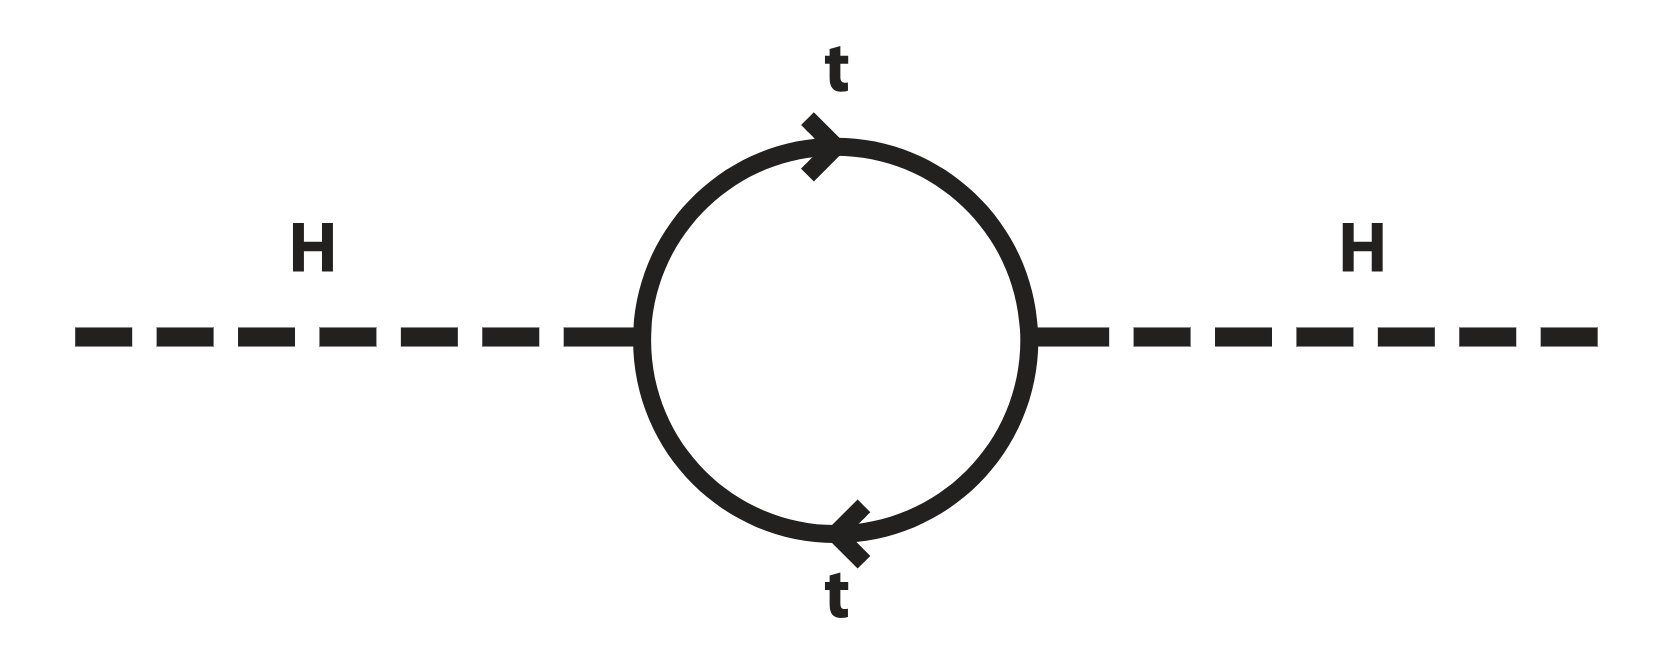
\includegraphics[width=0.6\linewidth]{susy_higgs_top_loop}
\caption{Top-quark loop diagram, the leading correction to the Higgs mass-squared. This contribution is quadratically divergent in the cutoff scale~\cite{susy-primer-1998}.}
\label{fig:susy_top_loop}
\end{figure}

The correction to the Higgs mass-squared coming from this diagram is~\cite{susy-primer-1998}:

\begin{equation}\label{eq:higgs_top_correction}
    \delta m_h^2 = \frac{3m_t^2}{2\pi^2 v^2}\Lambda_{UV}^2
\end{equation}

Where $m_t$ is the top quark mass, $v$ is the Higgs vacuum expectation value, and $\Lambda_{UV}$ is the ultraviolet cutoff.
Supersymmetry introduces a so-called superpartner for each Standard Model particle.
Standard Model fermions have bosonic superpartners, and Standard Model bosons have fermionic superpartners.
Superpartners always have the same quantum numbers as their Standard Model partners, except for spin.
The details of how this comes about will be discussed in~\ref{sec:susy_theory}.
The superpartner of the top is called the stop.
It's a scalar particle with all the same quantum numbers as the top quark, except for spin.

The introduction of superpartners leads to new quantum corrections to the Higgs mass-squared.
One of those corrections can be seen in~\ref{fig:susy_stop_loop}.

\begin{figure}[!ht]
    \centering
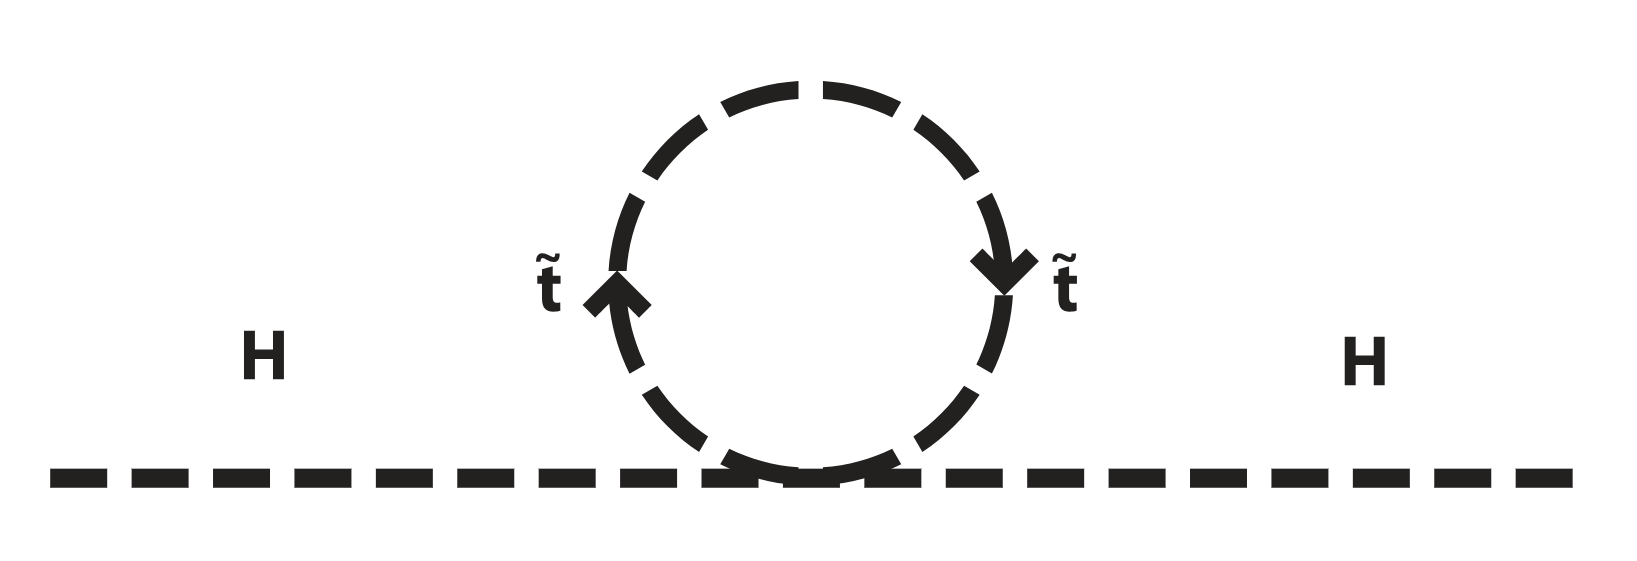
\includegraphics[width=0.6\linewidth]{susy_higgs_stop_loop}
\caption{Stop loop diagram, the leading SUSY correction to the Higgs mass-squared. This contribution is quadratically divergent in the cutoff scale~\cite{susy-primer-1998}.}
\label{fig:susy_stop_loop}
\end{figure}

The correction to the Higgs mass-squared coming from this diagram is~\cite{susy-primer-1998}:

\begin{equation}\label{eq:higgs_stop_correction}
    \delta m_h^2 = -\frac{3m_t^2}{2\pi^2 v^2}\Lambda_{UV}^2
\end{equation}

Thus, the quadratically-divergent top-loop correction is cancelled exactly.
A similar cancellation occurs for all other quadratic divergences in the calculation,
leaving terms that are only logarithmically divergent in the cutoff.

In SUSY, the leading correction to the Higgs mass-squared is proportional to the log of the cutoff scale,
and the squared difference between the top and stop masses~\cite{susy-pheno-2000}:

\begin{equation}\label{eq:susy_higgs_correction}
    \delta m_h^2 \propto \left(m_{\tilde{t}}^2 - m_t^2\right)  \Lambda_{UV}
\end{equation}

The amount of fine-tuning required can be quantified by $m_h / \delta m_h $, so in order to preserve naturalness,
the stop mass cannot be much heavier than the top quark mass.
If we allow for fine-tuning of only 1 part in 10, then the stop mass shouldn't be higher than the $1~TeV$ scale,
which indicates that SUSY should be accessible by the LHC .

Lower bounds on the masses of various suppersymmetric particles from ATLAS range from a few hundred $GeV$ to $2.4~TeV$~\cite{susy-summary-public}.
Figure~\ref{fig:susy_limits_summary} shows a sample of the SUSY particles and decay channels that have been searched for with ATLAS, and the resulting lower bounds.

\begin{figure}[!ht]
    \centering
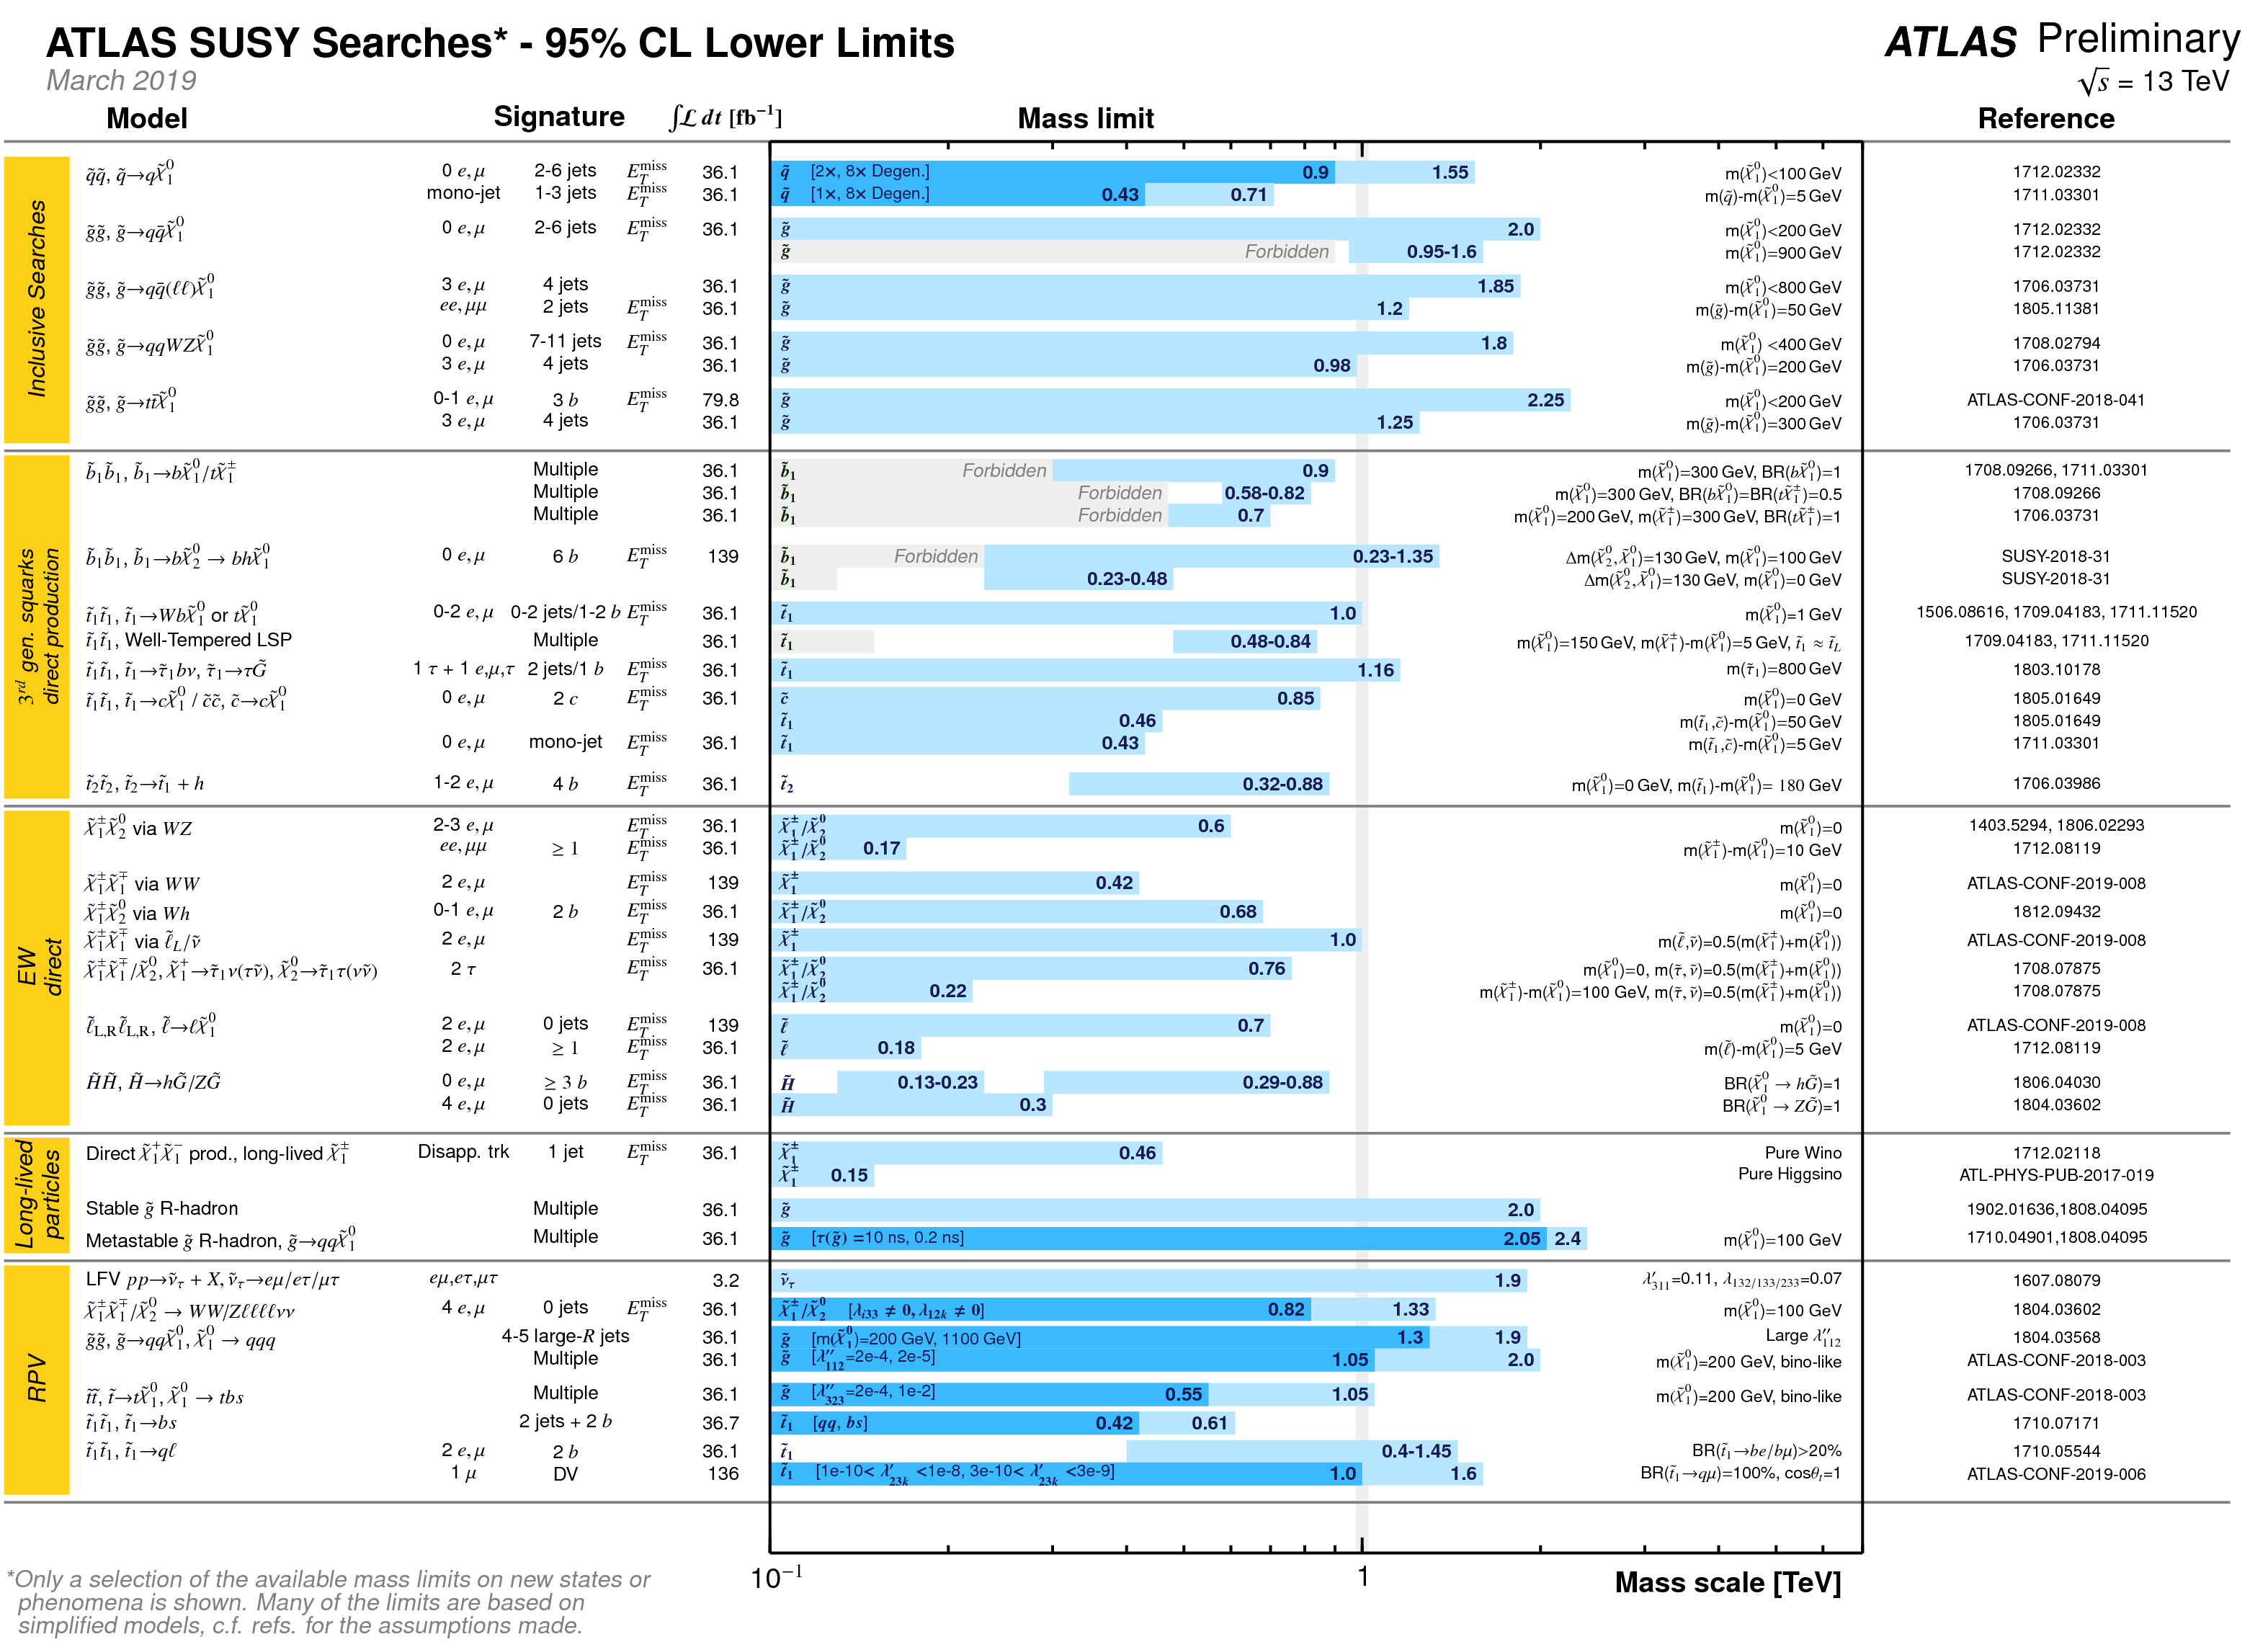
\includegraphics[width=1.1\linewidth]{susy_summary_limits.png}
\caption{A representative sample of the various SUSY searches performed by ATLAS, and their resulting mass lower bounds~\cite{susy-summary-public}.}
\label{fig:susy_limits_summary}
\end{figure}

\subsection{Grand Unification}\label{subsec:susy_unification}

Grand Unification is the idea that the $SU(3)_C \times SU(2)_L \times U(1)_Y$ symmetry of the Standard Model
could be embedded in a simpler symmetry group, which constrains the theory at energies above $\Lambda_{GUT}$.
In a Grand Unified Theory (GUT), there would be no distinction between quarks and leptons at energies above $\Lambda_{GUT}$,
and the differences in interactions between these two types of matter fields would be explained by the details of the
theory and the mechanism by which it is broken.
Furthermore, at energies above $\Lambda_{GUT}$, the three forces of the Standard Model would be replaced by a single, unified force.
Grand unification would be the logical next step after electroweak unification,
in which the electromagnetic and weak forces are shown to be the same force at energies above $\Lambda_{EW}\approx 246~GeV$.
Similarly to how electroweak unification gives a relationship between electric charge and weak isospin,
grand unification would give a relationship between color charge and the electroweak quantum numbers.

Several different symmetry groups have been proposed as GUTs.
Among these are $SU(5)$, $SO(10)$, $E_6$, and $SU(5)\times SU(5)$~\cite{susy-unification-1998}.
However, in order for unification to occur, the value of the three Standard Model coupling constants must converge at some energy scale.
The running of coupling constants is determined by the renormalization group equation (RGE):

\begin{equation}\label{eq:renorm_group}
    \frac{\partial g}{\partial \log \mu} = \beta(g)
\end{equation}

Where $g$ is the coupling constant of interest, $\mu$ is the energy scale at which the coupling is being measured,
and $\beta$ is a function that depends on the gauge structure and matter content of the theory.

Using the RGE, and measured values of the coupling constants at specific starting energies,
one can calculate the value of the three constants over a large range of energy scales.
It turns out that for the Standard Model, there is no energy scale at which all three Standard Model constants converge,
as would be required for a grand unified theory.

However, when the $\beta$ function is modified to include supersymmetric particles,
it is possible for all three Standard Model forces to unify.
In one particular SUSY model, known as the Minimal Supersymmetric Standard Model (MSSM),
unification of the forces occurs at $\mu \approx 2\times10^{16}~GeV$~\cite{susy-unification-1998}.
The running of the coupling constants under the Standard Model and MSSM can be seen in figure~\ref{fig:susy_unification}.

\begin{figure}[!ht]
    \centering
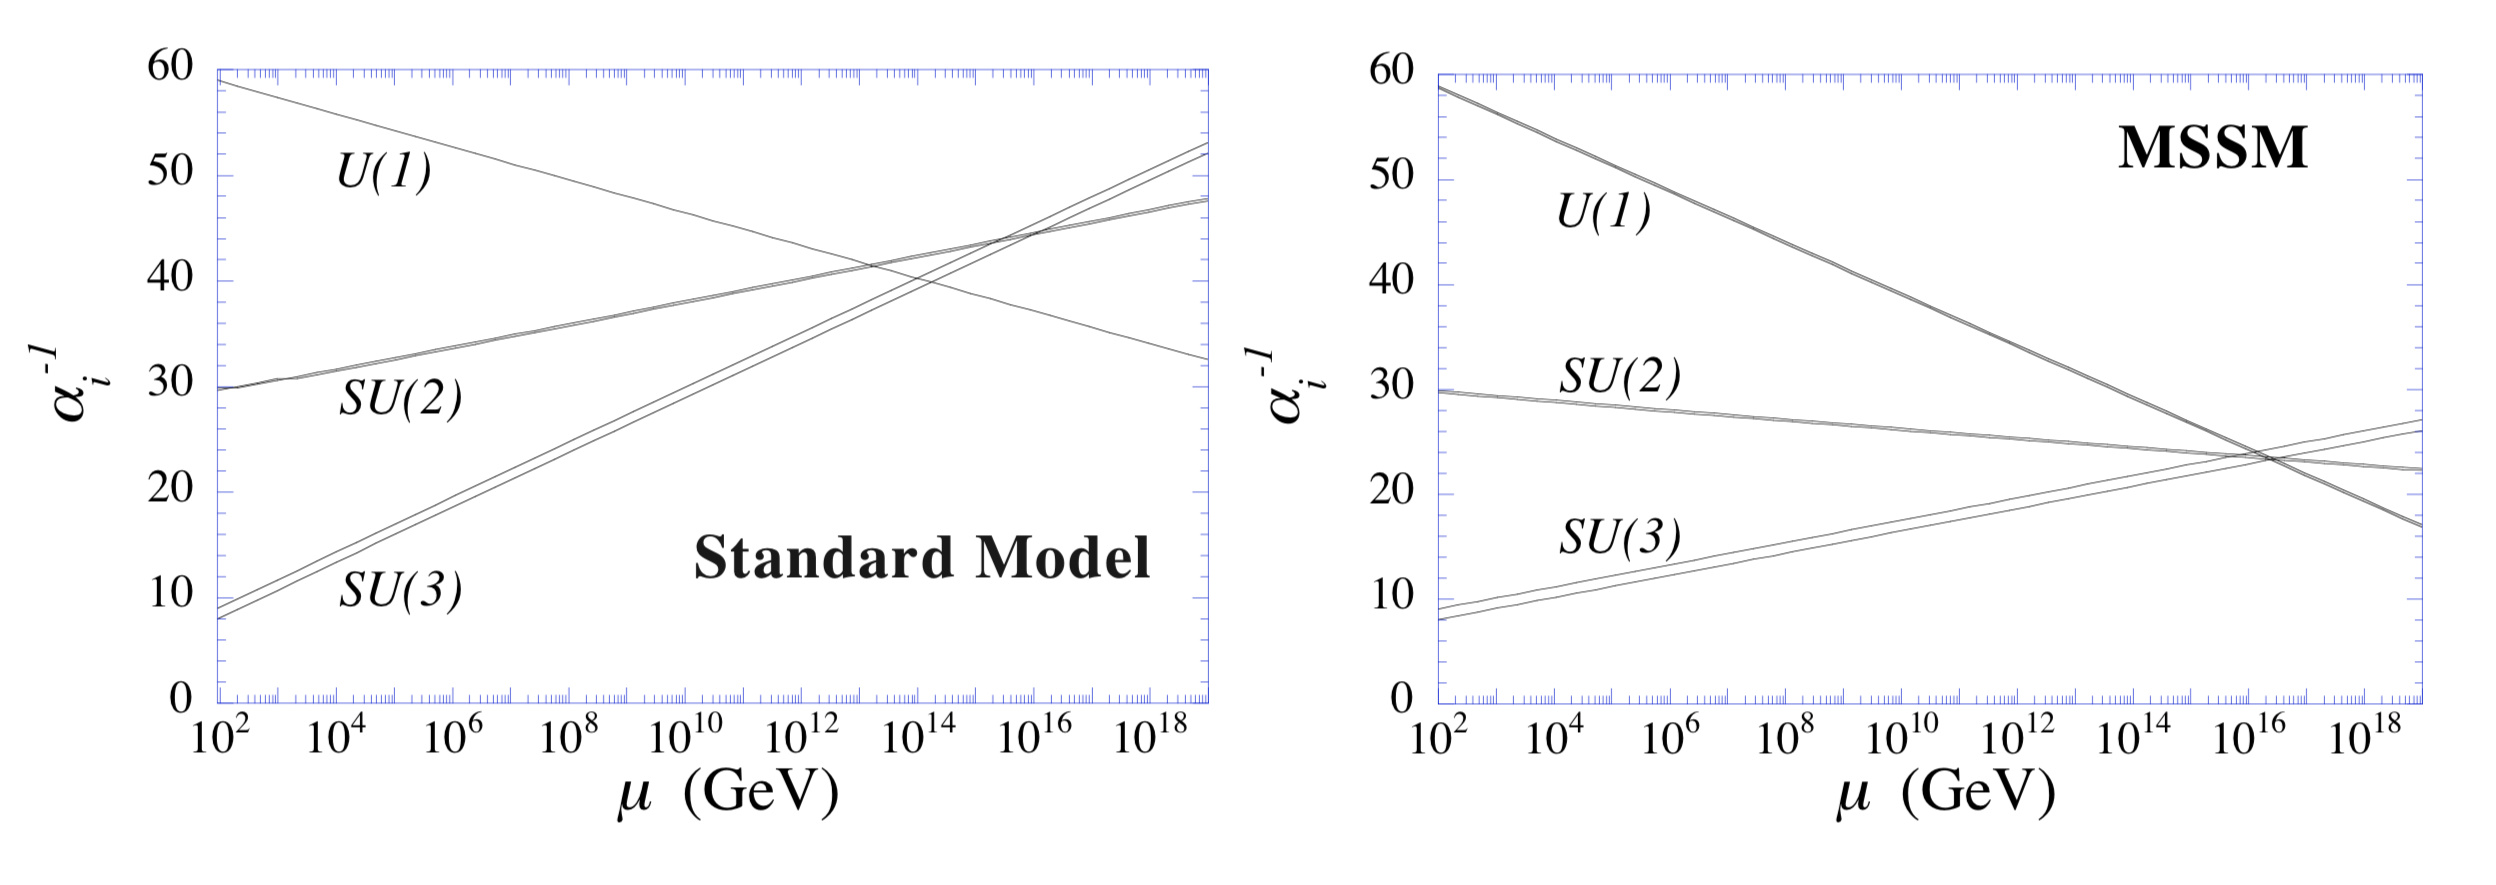
\includegraphics[width=0.95\linewidth]{susy_unification}
\caption{Running of the three Standard Model coupling constants under the Standard Model (left) and MSSM (right) RGEs.
For the MSSM, unification occurs at $\mu\approx 2\times 10^{16}~GeV$~\cite{susy-pheno-2000}.}
\label{fig:susy_unification}
\end{figure}

\subsection{Dark Matter}\label{subsec:susy_dark_matter}

As mentioned in~\ref{subsec:sm_dark_matter}, SUSY could explain Dark Matter,
which comprises approximately $80\%$ of matter in the universe, but still cannot be explained by any known particle.

In SUSY models that conserve R-parity\footnote{See section~\ref{sec:susy_rpv} for a discuss of R-parity and R-parity violation}, the lightest supersymmetric particle (LSP) must be stable because R-parity prevents the LSP from decaying to a final state without SUSY particles, and conservation of energy prevents it from decaying to a final state with SUSY particles.

In so-called "natural" SUSY, the LSP is a neutralino, $\chi_0^{1}$.
The neutralino is a mixture of the electroweak gauge superpartners, the wino and bino, and the Higgs superpartner, the higgsino.
The neutralino in this theory would be stable, massive, electrically neutral, and it would interact via the weak force.
As such, it is a viable candidate for WIMP dark matter.

Intriguingly, if one assumes that dark matter was thermally produced in the early universe,
and calculates the required production cross-section to match the dark matter abundance measured today,
the result is $\left<\sigma v\right> \approx 3 \times 10^{-26}~cm^{3}/s$,
which is very close to what would be expected for a weakly-interacting LSP~\cite{susy-dark-matter-1996}.

\section{Theory and Phenomenology}\label{sec:susy_theory}

Supersymmetry starts by positing a transformation that converts a boson field to a fermion field and vice versa,
and a Lagrangian which is invariant under such transformations.
Fields are represented in supermultiplets, which always contain a Standard Model particle and its superpartner.
Standard Model bosons are always paired with fermionic superpartners,
and Standard Model fermions are always paired with bosonic superpartners.
SUSY transformations commute with all symmetries of the Standard Model, except for the Lorentz transformations.
As a result, a Standard Model particle has all the same quantum numbers as its superpartner, except for spin.
Additionally, SUSY requires both members of the supermultiplet to have the same mass.
Experiments have ruled out the existence of same-mass superpartners for all Standard Model particles,
so for SUSY to be compatible with experimental evidence, it must be broken.
The method by which SUSY is broken should have an impact on the phenomenology of the model,
specifically on the differences in mass between the Standard Model particles and their superpartners.
A framework called soft SUSY breaking allows for the specifics of the SUSY breaking to be factored out,
by adding effective terms to the SUSY Lagrangian which account for the consequences of SUSY breaking without specifying the mechanism.
These new terms break SUSY explicitly, and so this is an effective field theory, valid only at energies well below the
SUSY-breaking scale~\cite{susy-soft-1981}.

\subsection{Superfields and superpotentials}\label{subsec:susy_superfields}
Superfields can be categorized into \textit{chiral} and \textit{gauge} superfields.
Standard model fermions and their superpartners will belong to chiral supermultiplets,
while Standard Model gauge bosons and their superpartners will belong to gauge supermultiplets.

A generic chiral superfield can be represented as $\Phi(x, \theta)$, where $x$ represents spacetime,
and $\theta$ denotes the additional two fermionic degrees of freedom needed for supersymmetry transformations.
It can alternatively be represented as $\Phi = \left(\phi, \psi \right)$, where $\phi$ is the complex scalar component,
and $\psi$ is the fermion component.

A generic \textit{vector} superfield can be represented at $V(x, \theta, \bar{\theta})$,
where $\bar{\theta}$ are the conjugate degrees of freedom to $\theta$.
In component form, vector supermultiplets can be represented as $V = \left(A^{\mu}, \lambda\right)$,
where $A^{\mu}$ is the gauge boson and $\lambda$ is the fermionic superpartner.

The generic supersymmetric action can then be written as~\cite{susy-unification-1998}:

\begin{equation}\label{eq:susy_action}
    S = \int d^4 x \int d^2 \theta d^2 \bar{\theta} \Phi^{\dagger} e^V \Phi
        + \int d^4 x \int d^2 \theta \left(W(\Phi) + W_{\lambda}(V)W_{\lambda}(V)\right)+h.c.
\end{equation}

Where the first integrand is the kinetic term for the matter fields,
and the second integrand contains the generic superpotential, $W(\Phi)$,
and the gauge kinetic term $W_{\lambda}(V)W_{\lambda}(V)$.

The function $W_{\lambda}(V)$ is defined as:

\begin{equation}\label{eq:susy_gauge_potential}
    W_{\lambda}(V) = \mathcal(D)^{2}\bar{\mathcal{D}}V
\end{equation}

where $\mathcal{D} \equiv \partial_{\theta}-i\sigma\dot \partial_x$~\cite{susy-unification-1998}.

\subsection{SUSY particles}\label{subsec:susy_mssm}
In the MSSM, the minimum number of new particles and free parameters are added to the already large assortment of Standard Model ones.
Each Standard Model fermion is paired with a spin-$0$ superpartner, and each Standard Model gauge boson is paired with a spin-$1/2$ superpartner.
For the Higgs boson, introducing a single superpartner is not enough.
There must be at least two Higgs chiral supermultiplets, with hypercharge values $1/2$ and $-1/2$.
This is needed in order to keep the electroweak theory anomaly-free, and for the Higgs mechanism to still give mass to all the fermions~\cite{susy-primer-1998}.

Superpartner states will be denoted with a tilde, and are also referred to as sparticles.
For example, the superpartner of the electron, called the selectron, will be denoted as $\tilde{e}$.

The MSSM chiral superfield content is summarized in table~\ref{tbl:susy_chiral_fields},
and gauge superfields are summarized in table~\ref{tbl:susy_gauge_fields}.

\begin{table}[!ht]
    \centering
  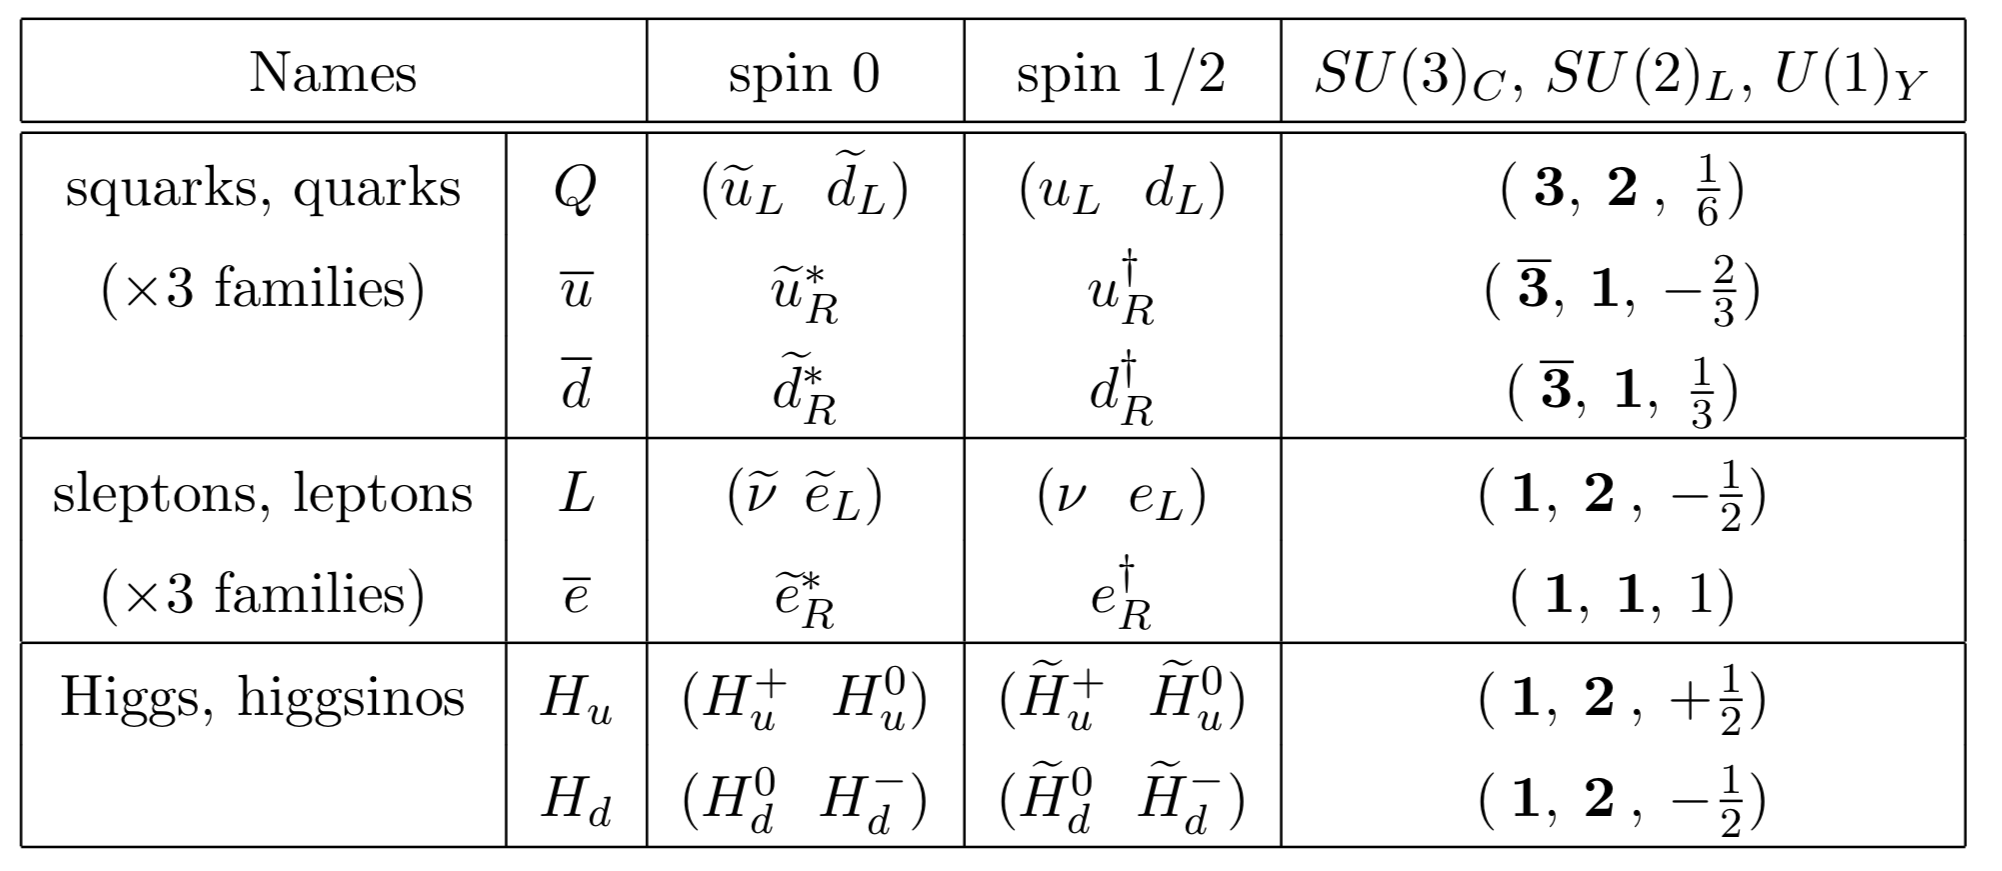
\includegraphics[width=\linewidth]{susy_chiral_superfields}
    \caption{The MSSM chiral superfields, including their names, symbols, and components.
  Quantum numbers for the Standard Model symmetry group transformations are also given~\cite{susy-primer-1998}.}
    \label{tbl:susy_chiral_fields}
\end{table}

\begin{table}[!ht]
    \centering

  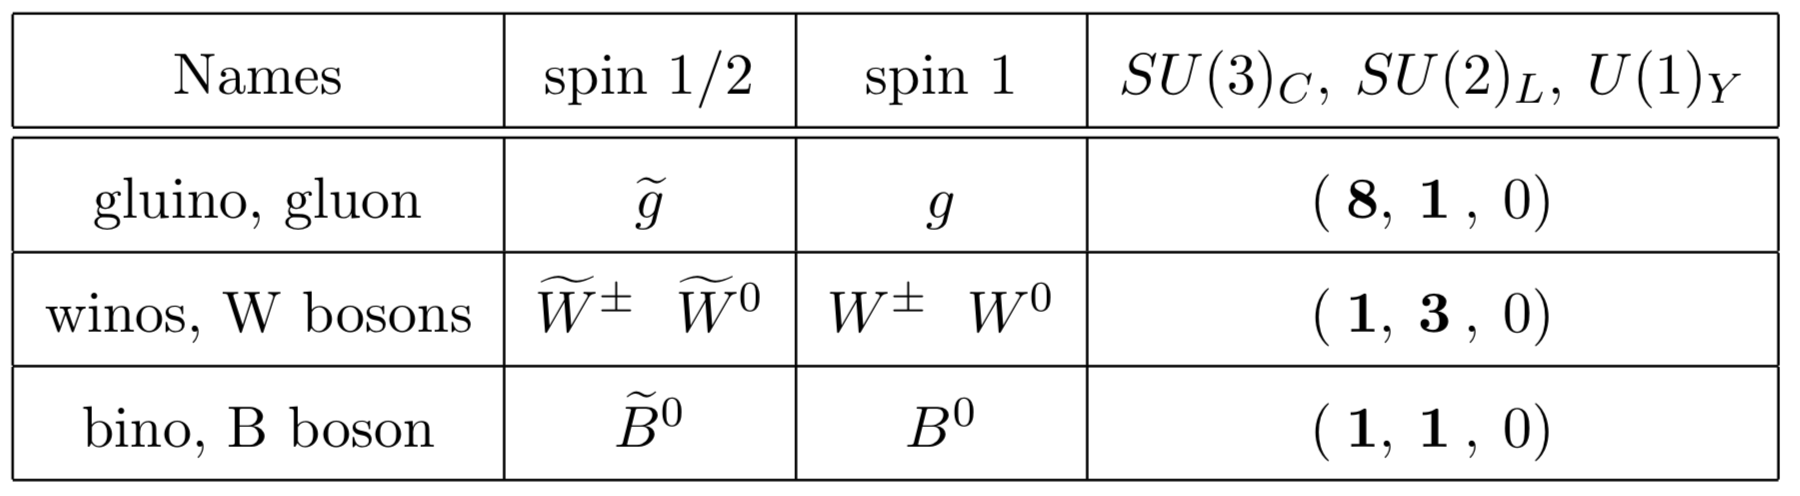
\includegraphics[width=\linewidth]{susy_gauge_superfields}
    \caption{The MSSM gauge superfields, including their names, symbols, and components.
  Quantum numbers for the Standard Model symmetry group transformations are also given~\cite{susy-primer-1998}.}\label{tbl:susy_gauge_fields}
\end{table}

The MSSM superpotential is then:

\begin{equation}\label{eq:susy_mssm_superpotential}
    W = h_l^{ij} e_i^c L_j H_d + h_d^{ij} Q_i d_j^c H_d + h_u^{ij} Q_i u_j^c H_u + \mu H_u H_d
\end{equation}

\noindent where all renormalizable terms that preserve the gauge symmetries, and are holomorphic in the chiral superfields have been included,
except for terms that violate baryon or lepton number conservation.
The indices $i, j, k$ are generation indices.
Here, the superpotential is expressed only in terms of the left-handed superfields and components,
and the hermitian conjugate terms are implied.

\section{R-Parity and R-parity Violation}\label{sec:susy_rpv}

In equation~\ref{eq:susy_mssm_superpotential}, certain terms were excluded from the superpotential because they
violate either baryon number or lepton number conservation.
But this requirement is in fact overly constraining.
While processes that violate baryon number or lepton number conservation have never been observed experimentally,
neither have they been ruled out.
Additionally, while there are no explicit B or L-violating terms in the Standard Model,
and no perturbative process in the Standard Model violates either,
there are in fact non-perturbative effects in the Standard Model which lead to violations of both~\cite{susy-bl-violation}.

\subsection{R-parity}\label{subsec:r_parity}

R-parity is a new symmetry which is introduced in order to eliminate the explicit B and L-violating terms from the
theory, without have to postulate that B and L are individually conserved.

Each particle has an R-Parity quantum number, defined as:

\begin{equation}\label{eq:r_parity_def}
    P_R = \left(-1\right)^{3\left(B-L\right)+2s}
\end{equation}

Where $B$ is the particle's baryon number, $L$ is its lepton number, and $s$ is its spin.
Quarks and squarks carry baryon number $1/3$, leptons an sleptons carry lepton number $1$,
and their corresponding antiparticles carry baryon number $-1/3$ and lepton number $-1$.

Every Standard Model particle has $P_R = +1$, and every sparticle has $P_R = -1$.

A necessary consequence of R-Parity conservation is the existence of a stable LSP .
In an R-parity-conserving (RPC) theory, interaction vertices that involve Standard Model particles cannot involve an odd number of sparticles.
As a result, when a sparticle decays, there must be at least one sparticle in the decay products,
in addition to any Standard Model particles.
So the lightest sparticle cannot decay, since there is no lighter sparticle for it to decay to.
Furthermore, in RPC SUSY, superpartners can only be produced in pairs at collider experiments,
since their production vertices necessarily include Standard Model particles.

\subsection{R-parity violating superpotential terms}\label{subsec:rpv}

If R-Parity conservation is not required, additional terms should be added to the MSSM superpotential.
Each term explicitly violates either baryon number or lepton number by one unit.
The R-Parity-violating (RPV) superpotential terms are:

\begin{equation}\label{eq:rpv_superpotential}
    W_{RPV} = \frac{1}{2} \lambda_{ijk} L_i L_j \bar{e}_k
    + \lambda'^{ijk} L_i Q_j \bar{d}_k + \mu'^i L_i H_u
    + \frac{1}{2} \lambda''^{ijk} \bar{u}_i \bar{d}_j \bar{d}_k
\end{equation}

Where $\mu'$, $\lambda$, $\lambda'$, and $\lambda''$ are new coupling constants.
The first three terms result in interaction vertices with $\Delta L = 1$,
and the last term is has $\Delta B = 1$.

\subsection{Rapid proton decay}\label{subsec:proton_decay}

In general, RPV SUSY would result in proton decay rates far higher than experimental bounds.
The main process leading to rapid proton decay requires both the $\lambda'$ and $\lambda''$ terms from equation~\ref{eq:rpv_superpotential}.
In this process, the proton decays to a $pi^0$ and a positron, via an off-shell squark.
The tree-level diagram leading to such a decay is shown in figure~\ref{fig:susy_proton_decay}

\begin{figure}[!ht]
    \centering
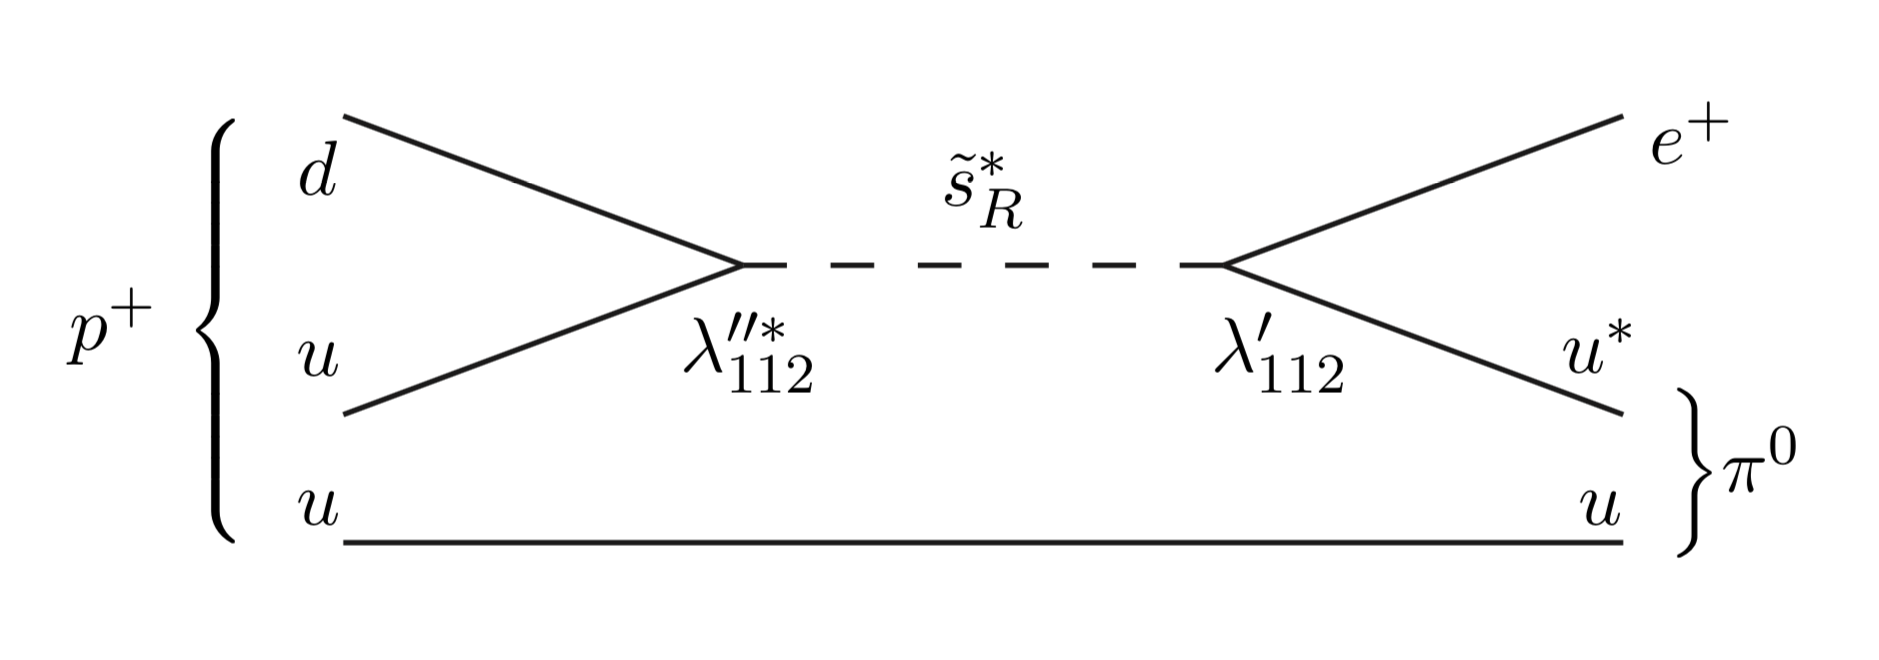
\includegraphics[width=0.95\linewidth]{susy_proton_decay}
\caption{Tree-level diagram for the decay $p^+ \rightarrow \pi^0 e^+$, with both L-violating and B-violating vertices~\cite{susy-primer-1998}.}
\label{fig:susy_proton_decay}
\end{figure}

The tree-level rate for this process is approximately~\cite{susy-primer-1998}:

\begin{equation}\label{eq:proton_decay_rate}
    \Gamma_{p^+ \rightarrow \pi^0 e^+} \sim \frac{m_p^5}{m_{\tilde{d}}^4} \sum_{i=2,3}\left|\lambda'^{11i}\lambda''^{11i}\right|^2
\end{equation}

Experimental bounds on the proton lifetime are greater than $10^{23}$ years,
so in order for RPV SUSY to be consistent with experiment,
either the squark masses have to be extremely large, or one of the couplings $\lambda'$, $\lambda''$ must be extremely small.

Specifically, the coupling and squark masses must satisfy~\cite{susy-rpv-constraints}:

\begin{equation}\label{eq:rpv_constraint}
    \lambda'_{11k} \lambda''_{11k} < 10^{-23} \left(\frac{m_{\tilde{q}}}{100~GeV}\right)^2
\end{equation}

For the search presented here, the ad-hoc assumption that $\lambda' = 0$ is made, in order to prevent predicted proton
decay rates inconsistent with experiment.

\subsection{R-parity violating gluino decays}\label{subsec:rpv_gluino}

The $\lambda''$ RPV term in the superpotential allows for two potential gluino discovery channels at the LHC.
The first involves pair-produced gluinos each decaying to three quarks via an effective vertex with an off-shell squark propagator.
This decay mode will be referred to as the direct decay model.

The second decay mode has the gluino first decaying to two quarks and an on-shell neutralino, via an RPC vertex,
and then the neutralino decaying to thre quarks through an effective RPV vertex,
which also includes an off-shell squark propagator.
This is the cascade decay model.

Diagrams for these two decay modes are shown in figure~\ref{fig:susy_rpv_decays}

\begin{figure}[ht!]
    \centering
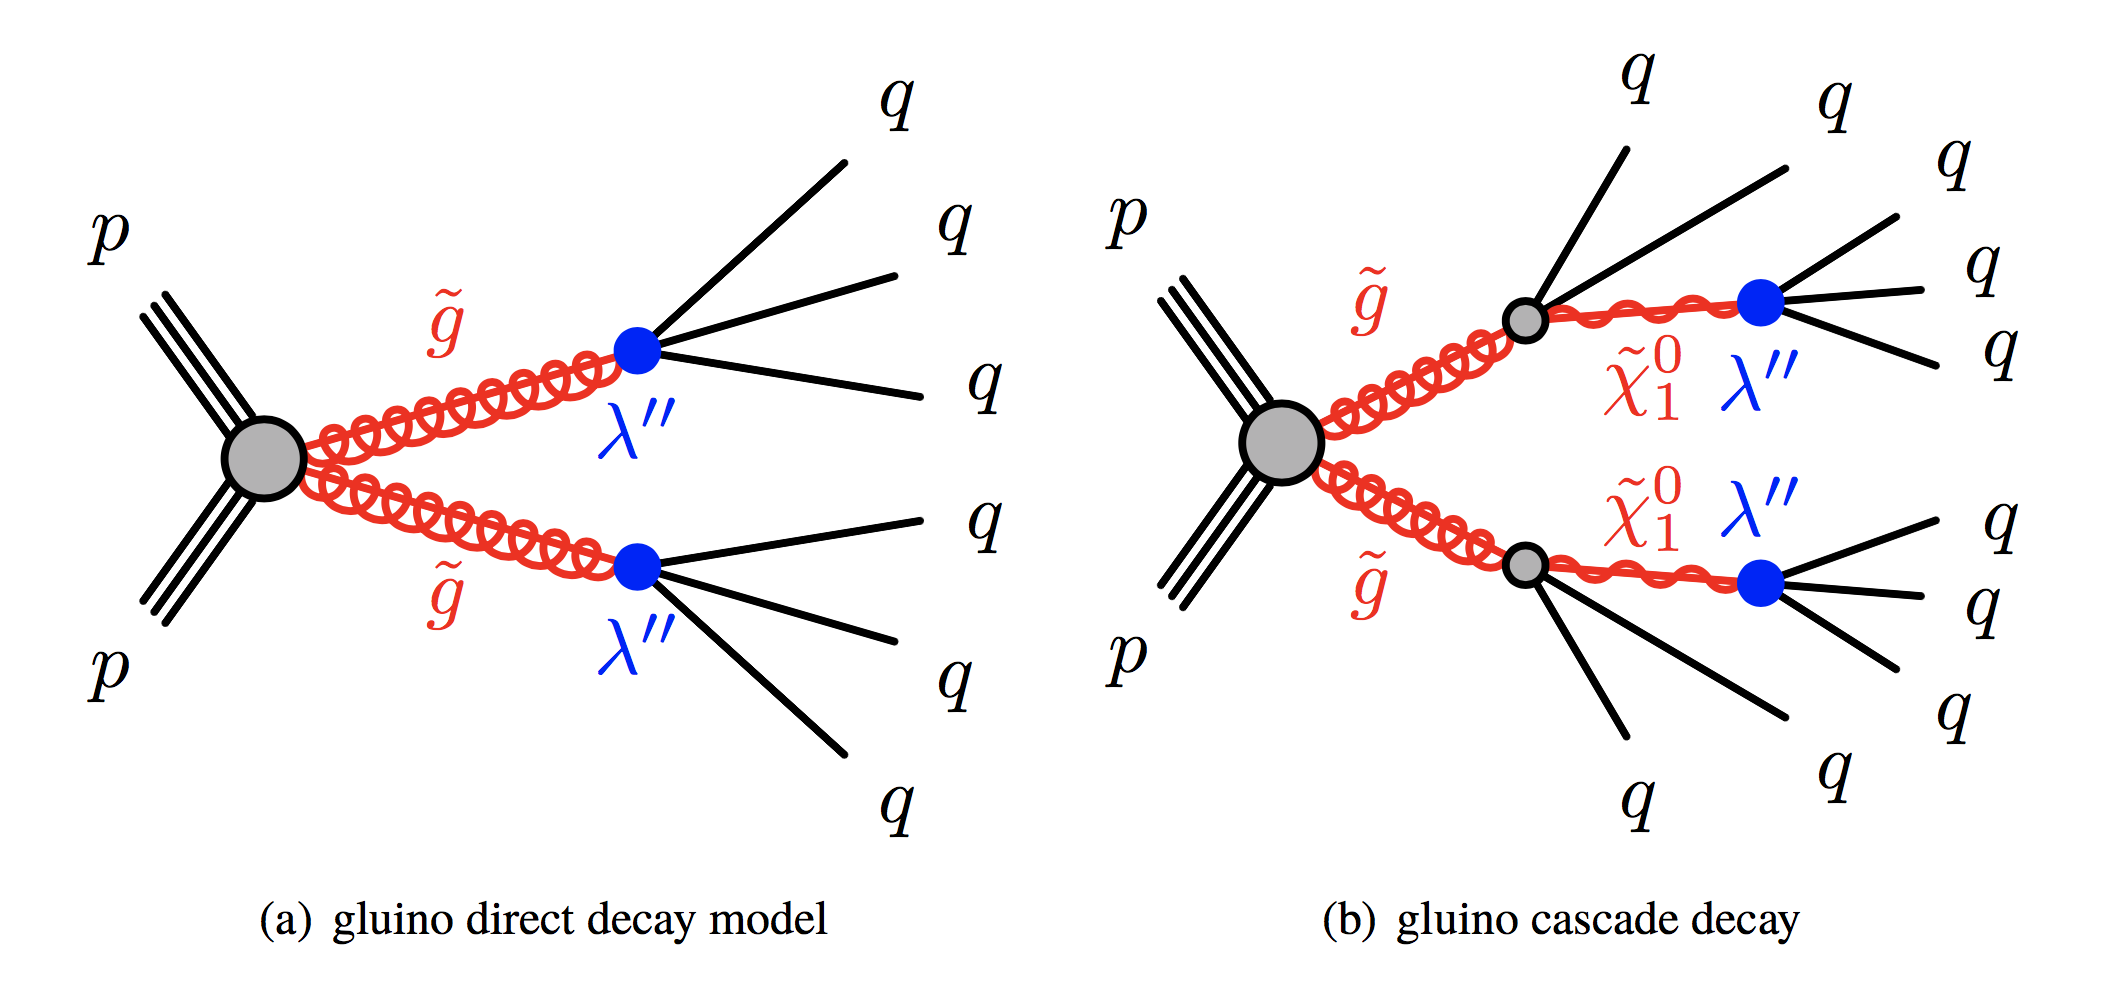
\includegraphics[width=0.95\linewidth]{decay_diagrams_combined}
\caption{Diagrams for the two decay processes that are the subject of this search. The direct decay (left) and cascade decay (right)
both involve effective RPV vertices containing off-shell squark propagators.}
\label{fig:susy_rpv_decays}
\end{figure}

Both decay modes result in a large number of high-momentum jets in the event.
The production and decay rates will depend on the values of the gluino mass, neutralino mass, and $\lambda''$.
A detailed discussion of the signal modeling is presented in chapter~\ref{ch:signal}.